\documentclass{article}
\usepackage{tikz}

\begin{document}

\centering

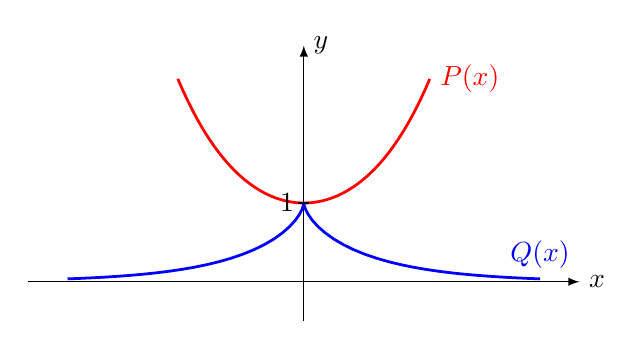
\begin{tikzpicture}
    % draw axes
    \coordinate (O) at (0,0);
    \draw[-latex] (0,-0.5) -- (0,3) node[anchor=west] {$y$};
    \draw[-latex] (-3.5,0) -- (3.5,0) node[anchor=west] {$x$};

    % draw curves
    \def\a{1} % constant
    \draw[red,domain=-1.6:1.6,samples=50, line width=1] plot ({\x},{\a*cosh(\x/\a)}) node[right] {$P(x)$};

    \draw[blue,domain=-4:4,samples=50, line width=1] plot ({\x - \a*tanh(\x/\a)},{\a/cosh(\x/\a)}) node[above] {$Q(x)$};

    % draw labels
    
    
    \node[anchor=east] at (0,1) {$1$};
    \draw (-2pt,1) -- (2pt,1);
    
\end{tikzpicture}

\end{document}